\documentclass[10 pt]{article}


\usepackage[latin1]{inputenc}
\usepackage[brazil]{babel}
\usepackage{enumerate}
\usepackage[autostyle]{csquotes}
\usepackage{graphicx}
\usepackage{hyperref}% to use \url{..} or \hyperref[label_name]{''link text''}
\renewcommand{\labelenumi}{\alph{enumi})}
\usepackage[autostyle]{csquotes}
%\input{unirioprojeto.tex}
\usepackage[final]{pdfpages}
%\usepackage{tabularx}
%\usepackage[table]{xcolor}
\usepackage{pdflscape}

\addtolength{\textwidth}{100pt} \addtolength{\textheight}{58pt}
\addtolength{\hoffset}{-50pt} \addtolength{\voffset}{-15pt}

%%%%%%%%%%%%%%%%%%%%%%%%%%%%%%%%%%%%%%%%%%%%%%%%%%%%%%%%%%%%%%%%%%%%%%%%
\providecommand{\U}[1]{\protect\rule{.1in}{.1in}}
%EndMSIPreambleData
\setlength{\topmargin}{-0.5 in} \setlength{\textwidth}{6.60 in}
%\setlength{\oddsidemargin}{0.2 in} \setlength{\evensidemargin}{0.2 in}
\setlength{\textheight}{9.6 in} \setlength{\marginparwidth}{0.5 in}
\setlength{\marginparsep}{0.5 in}
\renewcommand{\baselinestretch}{1.5}



\begin{document}

%    \titulo{Unirio de portas abertas}{2.2010}
%\includegraphics[scale=0.25]{unirio.png} %\includegraphics[scale=0.7]{faperj}

\begin{center}
{\large{\bf   Livro Aberto de Matemática}}
 \end{center}


    \section{Identificação do projeto}
\textbf{T\'itulo:} Livro Aberto de Matemática

\begin{flushright}
  \noindent
  \begin{tabular}{llll}
    &&\\
    &\textbf{Coordenadores:}& Fábio Luiz Borges Simas (UNIRIO)\\
    & & Augusto Quadros Teixeira (IMPA)

  \end{tabular}

\end{flushright}
\vspace{0.3cm}

\section{Resumo}

Este é um esforço de professores da Educação Básica e Superior, assim como de entusiastas, para produzir, até o final de 2017, uma coleção de livros didáticos de Matemática com código aberto, para o segundo ciclo do Ensino Fundamental, nos moldes do Plano Nacional do Livro Didático (PNLD).

A esta obra será atribuída a licença {\it Creative Commons} (CC) BY 4.0, isto significa que o material poderá ser livremente distribuído e alterado, mesmo que para fins comerciais.
Uma equipe vinculada ao projeto coordenará os esforços dessa tarefa.

O conteúdo dessa obra proverá de diversas fontes, após ser avaliada e adaptada pelo corpo de coordenadores.
Essas fontes incluem: contribuições da própria equipe de coordenadores, adaptações de Trabalhos de Conclusão de Curso (TCC) de graduação e mestrado, contribuições de professores e entusiastas e finalmente trabalhos disponibilizados com licenças compatíveis.

Espera-se que outros colaboradores ajudem na elaboração do material, aplicando os recursos em suas aulas, com comentários e até mesmo editando o material.
Esta cooperação se dará através de um site explicando a filosofia do projeto, onde será possível visualizar, baixar e comentar o texto já produzido.
Após cadastrar-se, o visitante também poderá editar o texto no próprio site, assim como na Wikipédia.
Com a diferença de que neste projeto todas as edições serão avaliadas pela equipe de revisão e a autoria de cada trecho do material será atribuída ao colaborador que a escreveu, desde que seja mantida a licença aberta do material.

\section{Introdução}

Recentemente o Brasil recebeu através do matemático Artur Avila a Medalha Fields, prêmio equivalente ao Nobel para matemática, conquistou a $34^a$ posição entre 109 países na $55^a$ Olimpíada Internacional de Matemática de 2014, que envolve jovens de até 19 anos.
Contudo, a realidade é outra quando voltam-se os olhos para o ensino básico. Na edição de 2012, o Brasil amarga uma das últimas posições no ranking de países que realizaram o PISA ({\it Programme for International Student Assessment}), que avalia estudantes de 15 anos a cada 3 anos mundo afora.
Esse resultado mostra que a educação matemática do brasileiro é desigual como a sociedade.
Enquanto apenas $1\%$ dos estudantes nesta idade consegue desenvolver e trabalhar com modelos em situações complexas, aproximadamente $67\%$ dos estudantes brasileiros nesta idade conseguem, no máximo, extrair informações relevantes de um texto e usar aritmética básica, fórmulas, procedimentos e convenções para resolver problemas envolvendo números \cite[Country Note - Brazil]{pisa2012} p. 2.

Existem diversos entraves para a melhoria do ensino nas escolas de Educação Básica dentre os quais destacam-se a qualidade na formação dos professores e a qualidade do livro didático adotado.
%Diversas medidas de longo prazo foram tomadas nos últimos anos para combater estes problemas.
Cabe ressaltar a interdependência deste dois aspectos quando \textquote{(...) o livro didático é, na maioria dos casos, a única fonte de referência do professor para organizar suas aulas, e até mesmo para firmar seus conhecimentos e dosar a apresentação que fará em classe.} (\cite{lima2001exame} p. 1). Isso acontece especialmente devido à posição de destaque que se encontra o livro didático na cultura educacional brasileira como observa \cite{machado}~p.~31

\blockquote{``(..) o livro `adotado' pelo professor - consumível ou não - praticamente determina o conteúdo a ser ensinado.
O professor abdica do privilégio de projetar os caminhos a serem trilhados, em consonância com as circunstâncias - experiências, interesses, perspectivas - de seus alunos, passando a conformar-se, mais ou menos acriticamente, com o encadeamento de temas propostos pelo autor.
 Tal encadeamento ora tem características idiossincráticas, ora resulta da cristalização de certos percursos, que de tanto serem repetidos, adquirem certa aparência de necessidade lógica; nos dois casos, a passividade do professor torna um pouco mais difícil a já complexa tarefa da construção da autonomia intelectual dos alunos.''}

 Claro que as formações de professores devem trabalhar para que o papel do professor e do livro didático na sala de aula sejam repensados tendo em vista o ensino como um processo pessoal, circunstancial e criativo.
 Contudo, não se pode negar o questionamento sobre a qualidade destes livros escolhidos pelas escolas.
 Sobre isso \cite{machado} p.~32 afirma que
 \blockquote{``(...) certamente existem livros de boa qualidade -- e nem sempre os mais adotados pelas escolas;
 o fato de os professores eventualmente escolherem aqueles que oferecem mais facilidades imediatistas do que recursos efetivos para um trabalho proveitoso em classe deve-se à cristalização de uma forma de utilização inadequada a que foram conduzidos, sobretudo, em razão de condições de trabalho reconhecidamente insatisfatórias.''}

De acordo com uma pesquisa realizada em Santa Maria - RS (ver \cite{zambon}) a escolha das coleções se inicia com a chegada de amostras das editoras e visitas de representantes, alguns gestores de escolas sequer sabem da existência do Guia do Livro Didático e os livros mais escolhidos costumam ser aqueles com maior trabalho de {\it marketing} realizado pelas editoras (visita de representantes e o envio de exemplares aos professores e às escolas).

Esta proposta surge para compor uma coleção de livros didáticos elaborados colaborativamente com participação dos próprios professores.
Na medida em que eles se tornem colaboradores, a escolha desta coleção será um movimento natural.

Dentre as características marcantes desta obra estará o compromisso com os objetivos do ensino de matemática no Ensino Fundamental (ver citação abaixo) presente na ideia de que mais importante do que os conteúdos a serem ensinados são as habilidades a serem desenvolvidas pelos estudantes.
Assim pretende-se estabelecer uma conversa com o professor a fim de responder às clássicas perguntas do estudante: {\it ``Onde vou usar isso na minha vida?''} ou {``\it Para que serve este conteúdo?''}.
Perguntas como essas costumam ser respondidas de maneira evasiva pelos professores.
Mas são perguntas pertinentes que os próprios professores deveriam se fazer ao prepararem suas aulas.
As respostas para costumam estar mais no modo de fazer do que no conteúdo em si.
Nesta proposta espera-se que os conteúdos ensinados aos estudantes tenham métodos sempre claramente identificados com os objetivos abaixo no livro do professor (Objetivos segundo o BNCC \cite{bncc} p.~121).

%Além disso, o professor se coloque numa postura mais criativa no processo de ensino em contraposição ao lugar de mero reprodutor do conteúdo na ordem e do modo que são apresentados no livro didático escolhido.

% Falar das áreas do BNCC (Geometria, Grandezas e Medidas, etc)

%Em maio de 2017 acontecerá no Rio de Janeiro a II International Conference on Mathematics Textbook Research and Development (ICTM2).
% A experiência dos programas Open Source.
%% Falar do OER Commons
%% Preço e qualidade dos livros didáticos aprovados no PNLD.
% (artigo do Nilson José Machado Em Aberto, Brasília, ano 16, n.69, jan./mar.
% 1996)
%% Escola e professores podem adaptar o texto para seus estudantes.
%%Professor deve se sentir autor do material para que dele se aproprie.
% BNCC e

% O BNCC determina alguns objetivos para o Ensino de Matemática na Educação Básica e mais especificamente no Ensino Fundamental.
%
 \blockquote{``OBJETIVOS GERAIS DA ÁREA DE MATEMÁTICA NO ENSINO FUNDAMENTAL \label{objetivosBNC}
\begin{itemize}
 \item Identificar os conhecimentos matemáticos como meios para compreender o mundo à sua volta.
 \item Desenvolver o interesse, a curiosidade, o espírito de investigação e a capacidade para criar/ elaborar e resolver problemas.
 \item Fazer observações sistemáticas de aspectos quantitativos e qualitativos presentes nas práticas sociais e culturais, sabendo selecionar, organizar e produzir informações relevantes, para interpretá-las e avaliá-las criticamente.
 \item Estabelecer relações entre conceitos matemáticos de um mesmo eixo e entre os diferentes eixos (Geometria, Grandezas e Medidas, Estatística e Probabilidade, Números e Operações, Álgebra e Funções), bem como entre a Matemática e outras áreas do conhecimento.
 \item Comunicar-se matematicamente (interpretar, descrever, representar e argumentar), fazendo uso de diferentes linguagens e estabelecendo relações entre ela e diferentes representações matemáticas.
 \item Desenvolver a autoestima e a perseverança na busca de soluções, trabalhando coletivamente, respeitando o modo de pensar dos/as colegas e aprendendo com eles/as.
 \item Recorrer às tecnologias digitais a fim de compreender e verificar conceitos matemáticos nas práticas sociocientíficas.''
\end{itemize}}

%
% Acreditamos que a democratização da educação passa pelo Open Source.
%
% Potencial para uso em outras disciplinas escolares.


\section{Relevância da proposta}

Ao ser construída com a filosofia {\it open source}, esta obra adquire um caráter permanente, de modo que independente dos organizadores, qualquer pessoa ou editora pode apropriar-se total ou parcialmente dos recursos nela disponíveis desde que respeitando os termos da licença. %(\url{http://creativecommons.org/licenses/by/4.0/deed.pt_BR}).

O preço de venda dos livros desta coleção não pode ser excessivo porque qualquer um pode editar e imprimir o mesmo material disponível no site.
Acredita-se que a ``Educação Aberta'' tenha potencial para readequar os preços dos livros didáticos brasileiros em um nível mais baixo.

Além da redução nos custos dos livros didático, esse projeto também visa melhorar a qualidade desses materiais.
Isso se dará através dos trabalhos de editoração e revisão feitos pela equipe coordenadora, assim como pela contribuição plural de diversos profissionais e entusiastas com formações e habilidades complementares.
Lembrando que outras coleções também podem se apropriar de trechos desta obra.

Apesar de toda a beleza desta iniciativa, de pouco ela vale se os professores das escolas decidirem não usufruir dos recursos disponíveis em nossos livros.
Neste sentido será fundamental a popularização e a divulgação massiva do material entre os professores das escolas ainda na fase de elaboração.
Na medida em que ele se torna autor ou colaborador da coleção, torna-se natural que a escolha para trabalhar com seus alunos.
Além disso, espera-se que o professor-autor adquira numa postura mais criativa no processo de ensino em contraposição ao lugar de mero reprodutor do conteúdo na ordem e do modo que são apresentados no livro didático escolhido.

\section{Objetivos}

\begin{enumerate}
\item Produzir uma coleção de livros didáticos de matemática com código aberto, de livre distribuição e edição contendo quatro volumes para os estudantes e quatro manuais de professores nos moldes do PNLD.
\item Melhorar a qualidade dos livros didáticos de matemática utilizados nas escolas públicas do segundo ciclo do Ensino Fundamental.
\item Reduzir os preços das coleções de livros de matemática concorrentes no PNLD para o segundo ciclo do Ensino Fundamental.
\item Conseguir adesão de diversos professores das escolas de Educação Básica para a ideia de {\it ``Educação Aberta''} e para esta coleção.
\item Estabelecer uma metodologia e plataforma de cooperação para produção de material didático que possa ser reproduzida em projetos análogos para outras disciplinas.
\end{enumerate}

% \section{Pontos críticos para o sucesso da obra}
%
% A qualidade e adesão desta coleção pelos professores dependerá principalmente de dois pontos: o comprometimento da equipe organizadora com a filosofia da coleção e do alcance que ela terá entre os professores no momento de sua elaboração.

 \section{A equipe}\label{equipe}

A equipe de 20 coordenadores do projeto será composta por um comitê de revisão e cinco comitês de elaboração (um para cada uma das áreas da matemática para este nível de escolaridade: Geometria, Grandezas e Medidas, Estatística e Probabilidade, Números e Operações, Álgebra e Funções).
Os comitês de elaboração deverão conter ao menos um professor dos anos finais do Ensino Fundamental (EF2).
Estes grupos podem contar com a colaboração de estudantes que trabalhem com os professores envolvidos.
Os participantes são especialmente encorajados a desenvolverem monografias de graduação e TCC do Profmat no contexto deste projeto junto com seus estudantes. %, embora não seja recomendada a participação formal no comitê de redação de estudantes do Profmat para que se evite o atraso no cronograma.
O comitê de revisão será formado por escritores renomados e, ao menos dois, professores experientes no EF2.

\clearpage
% \begin{table}[h]
% \begin{center}
% \begin{tabular}{ll}
% PROFESSORES UNIVERSTÁRIOS            & PROFESSORES DA EDUCAÇÃO BÁSICA  \\
% Humberto Bortolossi - UFF            & Leo Akio - CAp UFRJ\\
% Gladson Antunes - UNIRIO             & Felipe Ferreira - SESC e Colégio Santo Ignácio\\
% Michel Cambrainha - UNIRIO           & Eduardo Wagner - FGV  \\
% Victor Giraldo - UFRJ                & Luiz Felipe Lins - Prefeitura do Rio de Janeiro\\
% Alexandre Silva - UNIRIO             & \\%Letícia Guimarães Rangel - CAp da UFRJ
% Wanderley Resende - UFF              & Priscila Guez - Prefeitura do Rio de Janeiro\\
% Fabio Simas - UNIRIO (elaborador)    & \\%Sérginho - CP2 (revisor)
% %Luciane Velasque - Unirio (elaboradora) & %Sérginho - CP2 (revisor)
% \end{tabular}
% \end{center}
% \end{table}
% {\centering Obs.: A equipe acima ainda não têm a participação confirmada e outros não listados deverão compor a equipe.}


\noindent{\it Responsabilidades de cada membro na equipe.}

 \begin{enumerate}[A.]
  \item Elaborador
  \begin{enumerate}[(1)]
   \item Escrever material para os livros.
   \item Buscar material que julgue de qualidade, contactar os autores para apresentação do projeto e solicitar atribuição de licença CC BY 4.0. Efetuar as adaptações necessárias antes de submeter à equipe de revisão.
   \item Apresentar sua produção neste projeto nos encontros mensais da equipe.
   \item Colaborar com os revisores discutindo e implementando as sugestões dadas.
   \item Colaborar com os membros de outros comitês de elaboração propondo métodos de abordagens e tópicos extras para a composição dos volumes.
   \item Orientar estudantes em nível de graduação e mestrado em monografias que podem compor trechos dos livros (quando professor universitário).

  \end{enumerate}

  \item Revisor:
  \begin{enumerate}[(1)]
  \item Analisar a relevância para a coleção do texto submetido.
  \item Analisar a consistência matemática do texto submetido.
  \item Verificar se as habilidades desenvolvidas contemplam aquelas da BNCC.
  \item Verificar se os pré-requisitos para o conteúdo já foram trabalhados.
  \item Corrigir o uso da norma culta.
  \item Efetuar a adequação da linguagem para o Ensino Fundamental (quando professor da Educação Básica).
  \end{enumerate}

   \item[B.1.] Revisor de área
   \begin{enumerate}
\item[(8)] Verificar se há saltos no nível de dificuldade do material daquela área.
   \end{enumerate}

  \item[B.2.] Revisor de ano letivo
  \begin{enumerate}
\item[(8)] Verificar se há saltos no nível de dificuldade no conteúdo daquele ano.
\item[(9)] Avaliar se a extensão do texto supera o limite estipulado para aquele ano.
  \end{enumerate}
  \end{enumerate}



\section{Método}
\label{metodo}

O projeto será apresentado em um site na internet, onde poderão ser visualizados e baixados o sumário de cada livro e os capítulos da coleção em suas versões mais recentes.
Haverá um espaço para comentários sobre o conteúdo de cada capítulo.
O usuário poderá editar o texto diretamente, assim como na Wikipédia.
Para isso deverá se registrar e concordar com os termos da licença.
Então com um clique acessará um editor de textos com o código em {\it latex} do capítulo que está visualizando.
Ao término da edição, o revisor de área será informado das alterações linha por linha.
Estas modificações somente serão incorporadas ao texto disponível para visualização após a concordância deste revisor.
O revisor de ano deve ter uma visão mais global do trabalho e possuirá uma postura mais ativa efetuando uma segunda leitura crítica de cada parte do texto. Os frequentes comentários dos revisores devem ser um termômetro do bom andamento do projeto.

O aparato tecnológico necessário já existe, falta apenas a junção de ferramentas para que a cooperação seja o mais simples possível.
Na seção do site em que figura a visualização de dado arquivo, haverá link para o código-fonte do arquivo no {\it GitHub} (servidor de arquivos com serviço de compartilhamento e controle de versões já utilizado para projetos como este, por exemplo, neste servidor é desenvolvido o Linux).
O {\it GitHub} informa as alterações feitas pelo usuário aos revisores.
O funcionamento destes recursos bem como a aderência dos comitês de elaboração e revisão à esta tecnologia será testada e poderá sofrer alterações antes da divulgação ao grande público.

O conteúdo desta obra será aquele determinado pela Base Nacional Comum Curricular (ver Anexo \ref{habilidades}) complementado com alguns tópicos extras a serem selecionados pela equipe organizadora.
A produção inicial ficará a cargo de TCC de graduação e do Profmat sob a orientação dos professores envolvidos, também serão incorporados alguns trabalhos já existentes de autores que aceitem disponibilizá-los nos termos da licença desta coleção.
Além disso, qualquer pessoa que tenha interesse, pode editar o texto, modificando, excluindo ou adicionando novos trechos.

Todos os membros da equipe organizadora se reunirão mensalmente com os seguintes objetivos principais:
\begin{itemize}

 \item Escolha de quais dos ``Objetivos Gerais da Área de Matemática no EF2'' (ver p. \pageref{objetivosBNC}) devem ser atingidas nos diversos tópicos que serão abordados (este item pode ser discutido em separado pelos comitês de elaboração com um revisor e depois apresentado aos demais para discussão).
 \item Definição de metas de elaboração para o próximo mês.
 \item Determinação das habilidades extras (aquelas que não figuram no BNCC) que serão incorporadas ao texto de cada volume.
 \item Discussão metodológica para abordagem de cada um dos tópicos, como obter inter-relação com as outras 4 áreas da matemática para este nível de escolaridade (Geometria, Grandezas e Medidas, Estatística e Probabilidade, Números e Operações, Álgebra e Funções) e outras áreas do conhecimento.
 \item Definição do número de páginas por área no respectivo volume.
 \item Apresentação do andamento do trabalho dos comitês de elaboração.
 \item Unificação da linguagem do texto.
 \item Colaboração de toda a equipe com o trabalho de cada comitê de elaboração.
 \item Aproximação de revisores e elaboradores.
\end{itemize}

\clearpage

Na  Seção \ref{cronograma} estão os prazos e estruturação lógica das etapas descritas abaixo.

\begin{enumerate}
\item[Fase 1 -] {\it Estruturação do ambiente virtual de desenvolvimento e organização das equipes.}

Este é o momento para desenvolver o aparato tecnológico necessário ao projeto, recrutar e treinar a equipe para o uso destes recursos.
Aqui serão definidas preliminarmente as funções de cada membro da equipe e divisão de áreas entre os comitês de elaboração.
Esta fase termina quando cada participante souber suas atribuições (preliminares), estiver capacitado para utilizar a tecnologia necessária à sua participação e os comitês de elaboração já tiverem definidos as suas metas de habilidades do BNCC para o volume do sexto ano.

\item[Fase 2 -] {\it Consolidação do ambiente virtual de desenvolvimento, redação, revisão e teste do volume do sexto ano.}

Nesta etapa o volume do sexto ano terá sua primeira versão finalizada. Entende-se por ``volume'' o livro do estudante e o respectivo manual do professor.
Os comitês de elaboração manterão seu progresso atualizado no site, permitindo deste modo que os revisores acompanhem e comentem seu desenvolvimento semanalmente.
Durante esta fase será realizada a revisão de todo primeiro volume.
Os comitês de elaboração podem ser convidados a reescrever ou realizar adaptações pelo comitê revisor, que também poderá editar o material diretamente.
Após esta fase o comitê revisor ainda avaliará sugestões de alteração neste volume.
Somente até esta fase a interface do recurso computacional para controle de versões e colaboração poderá ser modificada consideravelmente.
Daqui para frente apenas alterações suaves na interface devem acontecer.
A equipe organizadora solicitará aos estudantes do Profmat que experimentem as atividades com seus estudantes do sexto ano e que colaborem compartilhando suas impressões sobre as partes utilizadas do volume bem como suas impressões sobre o uso da tecnologia.
%A pertinência dos comentários será avaliada pelo comitê de revisores.
A conclusão desta fase se dará quando o comitê de revisão decidir que existe uma primeira versão final para o Volume 1 desta obra e e quando estiver finalizado o ambiente virtual de colaboração.


\item[Fase 3 -] {\it Divulgação do material, redação, revisão e experimentação do volume do sétimo ano.}

Este é o momento em que o projeto alcança grande visibilidade entre os professores de matemática. Serão utilizados sites de organizações consagradas para a divulgação do material (e.g. OBM, OBMEP, SBM, Profmat, CDME, SBEM, SBE, UFRJ, UFF, Unirio).
Desse modo espera-se obter diversos colaboradores para testar, revisar, opinar e editar os volumes daqui para frente.
A partir deste momento a equipe coordenadora do projeto deve aproveitar as oportunidades que tiver para participar de atividades ou eventos pelo Brasil em que tenha oportunidade de apresentar o projeto a professores do EF2.

%\item[Fases 4, 6 e 8 -] {\it Redação dos volumes do sétimo, oitavo e nono ano, respectivamente.}

%\item[Fases 5, 7 e 9 -] {\it Experimentação e revisão dos volumes do sétimo, oitavo e nono ano, respectivamente.}

\item[Fase 4 -] {\it Redação, revisão e experimentação do volume do oitavo ano.}

\item[Fase 5 -] {\it Redação, revisão e experimentação do volume do nono ano.}

\item[Fase 6 -] {\it Revisão da coleção e entrega à editora.}
\end{enumerate}








%\subsection{Da experimentação do material}

%\subsection{Dos direitos autorais e da licença}

%{\it Creative Commons 4.0} %\url{http://creativecommons.org/licenses/by/4.0/deed.pt_BR}

%\subsection{Da editoração}

%Todo o trabalho de diagramação, impressão e editoração será realizado pelo IMPA.

%\clearpage
\section{Cronograma de execução}\label{cronograma}

O cronograma de execução das tarefas do projeto bem como seu encadeamento lógico estão na Figura \ref{tarefas}:

\begin{landscape}
\begin{figure}[ht]
 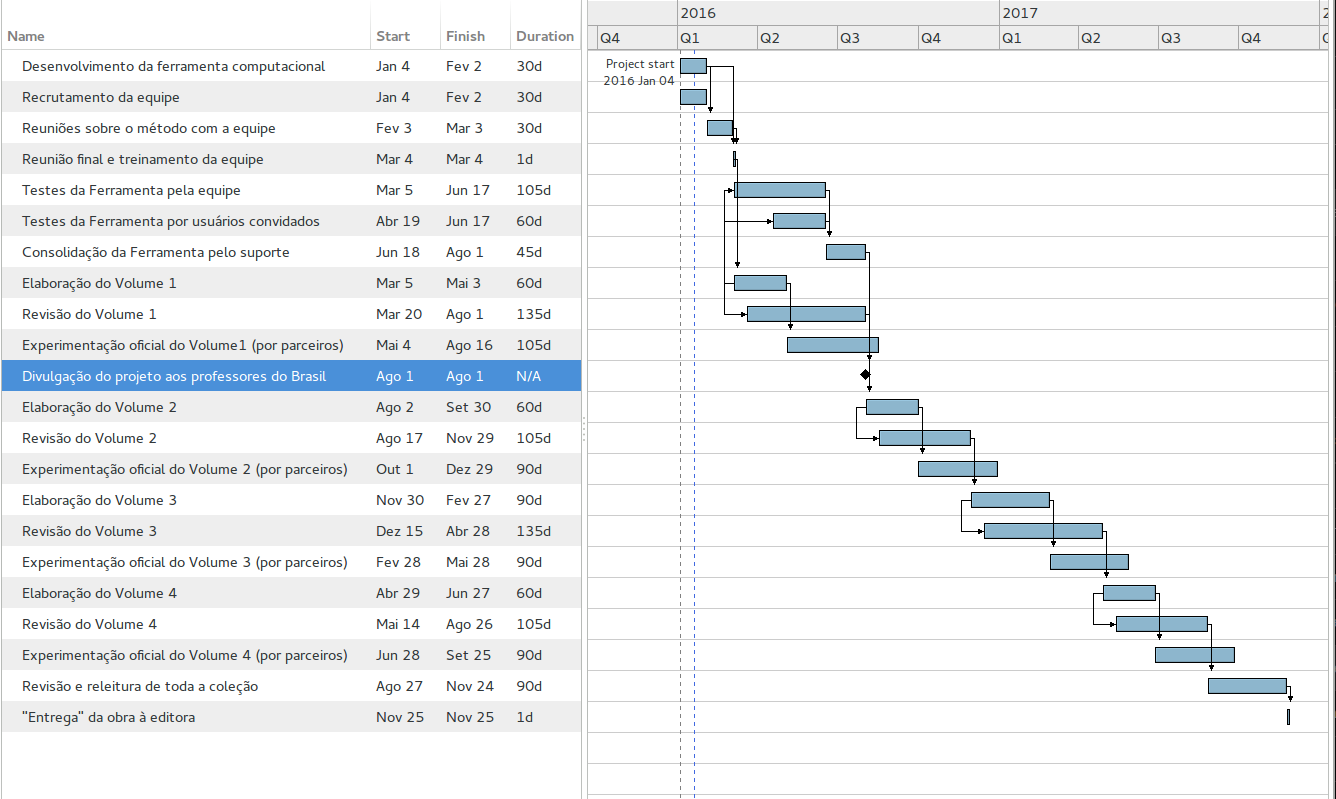
\includegraphics[width=\paperwidth,]{estrutura_das_tarefas}
 \caption{Estruturação das tarefas e prazos para execução} \label{tarefas}
\end{figure}
\end{landscape}

\section{Recursos financeiros}

Todo o suporte técnico necessário a esta proposta será disponibilizado pela Organização Social Instituto Nacional de Matemática Pura e Aplicada (IMPA-OS). Para que se obtenha a dedicação esperada da equipe organizadora desta proposta e para que ocorram as viagens descritas na Metodologia serão necessários recursos conforme a tabela a seguir:

\begin{table}[h] \label{tab pessoal}
  \begin{center}
\begin{tabular}[h!]{|l|c|}
   \hline
%\rowcolor{lightgray}
\multicolumn{2}{|c|}{{\bf DESPESAS DE CUSTEIO: Elaboradores e revisores}} \\
   \hline
   Quantidade de pessoas & 20\\
   \hline
   Custo mensal unitário & R$\$$ 1.300,00\\
   \hline
    Custo mensal total & R$\$$ 26.000,00\\
   \hline
   {\bf Total} & {\bf R$\$$ 624.000,00} \\
   \hline
\end{tabular}
  \end{center}
  \caption{Despesas de Custeio com Pessoal}
 \end{table}

\begin{table}[h] \label{tab viagens}
  \begin{center}
\begin{tabular}[h!]{|l|c|}
   \hline
%\rowcolor{lightgray}
\multicolumn{2}{|c|}{{\bf DESPESAS DE CUSTEIO: Viagens}} \\
   \hline
   Quantidade de viagens & 24\\
   \hline
   Custo unitário médio de passagem & R$\$$ 1.000,00\\
   \hline
   Quantidade de diárias por viagem & 3\\
   \hline
   Valor da diária & R$\$$ 600,00\\
   \hline
   {\bf Total} & {\bf R$\$$ 67.200,00} \\
   \hline
\end{tabular}
  \end{center}
  \caption{Despesas de Custeio com Viagens}
 \end{table}

 \begin{table}[h!]\label{tab orcamento}
  \begin{center}
   \begin{tabular}{|c|c|}
   \hline
   \multicolumn{2}{|c|}{{\bf ORÇAMENTO TOTAL}} \\
   \hline
   RUBRICAS &  Valor Total (R$\$$)\\
   \hline
   Custeio de pessoal &  R$\$$ 624.000,00 \\
   \hline
   Custeio de viagens &  R$\$$ 67.200,00 \\
   \hline
   {\bf TOTAL}&{\bf R$\$$ 691.200,00}\\
   \hline
   \end{tabular}
  \end{center}
  \caption{Orçamento Total}
 \end{table}
% \begin{table}[ht]
% \begin{center}
% \begin{tabular}{ccccccccccccc}
% 2016 & Jan & Fev & Mar & Abr & Mai & Jun & Jul & Ago & Set & Out & Nov & Dez \\
% 	\hline
% Fase 1  & $\bullet$ &  $\bullet$ & & &  \\
% \hline
% Fase 2 & & & $\bullet$ & $\bullet$ &  & &  \\
% \hline
% Fase 3 & & & & & $\bullet$ & $\bullet$ & $\bullet$ &\\
% \hline
% Fase 4 & & & & & & & & $\bullet$ & $\bullet$  & &\\
% \hline
% Fase 5& & & & & & &  &  &  &$\bullet$ & $\bullet$ &\\
% \hline
% Fase 6& & & & &  &  &  &  &  &  & & $\bullet$ \\
% \hline
% \end{tabular}
%   \end{center}
%   \end{table}
%
% \begin{table}[ht]
% \begin{center}
% \begin{tabular}{ccccccccccccc}
% 2017 & Jan & Fev & Mar & Abr & Mai & Jun & Jul & Ago & Set & Out & Nov & Dez \\
% 	\hline
% Fase 6  & $\bullet$ & $\bullet$ &  & & &  \\
% \hline
% Fase 7 & & & $\bullet$ & $\bullet$ &  & &  \\
% \hline
% Fase 8 & & & & & $\bullet$ & $\bullet$ &\\
% \hline
% Fase 9 & & & & & & & $\bullet$ & $\bullet$ & $\bullet$ &\\
% \hline
% Fase 10& & & & & &  &  &  &$\bullet$ & $\bullet$ & $\bullet$ & $\bullet$ \\
% \hline
% \end{tabular}
% \end{center}
%   \end{table}
%
%

%\vspace{6 cm}
%
% \begin{flushright}
%   Rio de Janeiro, 12 de janeiro de 2016
% \end{flushright}
%
% \vspace{6 cm}

% estilo da bibliografia
\bibliographystyle{apalike}
% chamando o arquivo refs.bib
 \bibliography{refs}
\clearpage

% \appendix
% \section{Habilidades do BNCC para o sexto ano}\label{habilidades}
% 
% {\it Geometria.} \newline
% MTMT6FOA001 Associar pares ordenados a pontos do plano cartesiano, considerando apenas o primeiro quadrante.\newline
% MTMT6FOA002 Diferenciar polígonos de não polígonos, classificando-os como regulares e não regulares.\newline
% MTMT6FOA003 Reconhecer características dos quadriláteros, classificando-os em relação a lados e a ângulos.\newline
% MTMT6FOA004 Construir figuras planas semelhantes em situações de ampliação e redução, reconhecendo a conservação dos ângulos e a proporcionalidade entre os lados, usando malhas ou tecnologias digitais.\newline
% MTMT6FOA005 Desenhar retas paralelas e perpendiculares, usando instrumentos de desenho.
% 
% \noindent{\it Grandezas e Medidas.}\newline
% MTMT6FOA006 Resolver e elaborar problemas, sem o uso de fórmulas, envolvendo noções de medida de comprimento, área (triângulos e retângulos), massa, capacidade, volume (blocos retangulares) e temperatura, aplicando as relações entre as unidades de medida mais usuais.\newline
% MTMT6FOA007 Determinar medida de ângulos, com uso de transferidor ou tecnologias digitais.\newline
% MTMT6FOA008 Reconhecer que perímetro e área são independentes e descrever o que ocorre com as medidas do perímetro e da área de um quadrado ou de um retângulo, quando se altera a medida de seus lados (exemplo: dobra, triplica).
% 
% \noindent{\it Estatística e Probabilidade.}\newline
% MTMT6FOA009 Indicar a probabilidade de um evento por um número racional (na forma fracionária, decimal e percentual) e compreender que, se um experimento aleatório for realizado com um grande número de tentativas, os resultados obtidos tendem à probabilidade calculada.\newline
% MTMT6FOA010 Reconhecer os elementos de um gráfico de colunas, barras e linha (eixos, título, fonte e legenda).\newline
% MTMT6FOA011 Comparar e interpretar dados de uma pesquisa que envolve duas categorias de variáveis, apresentadas por meio de colunas agrupadas.
% 
% \noindent{\it Números e Operações}\newline
% MTMT6FOA012 Classificar números de diferentes magnitudes em pares e ímpares, primos e compostos e compreender relações entre números (expressas pelos termos ``é múltiplo de''; ``é divisor de''; ``é fator de'') e critérios de divisibilidade por 2, 3, 4, 5, 6, 8, 9 e 10.\newline
% MTMT6FOA013 Identificar e registrar números racionais positivos em suas diferentes representações, identificando equivalências e passando de uma representação para outra.\newline
% MTMT6FOA014 Comparar e ordenar números naturais e racionais positivos (representação fracionária e decimal), relacionando-os a pontos na reta numérica.\newline
% MTMT6FOA015 Resolver e elaborar problemas envolvendo as ideias de múltiplos, divisores, mínimo múltiplo comum, máximo divisor comum.\newline
% MTMT6FOA016 Resolver e elaborar problemas, envolvendo as quatro operações fundamentais, com seus diferentes significados, com números naturais, inclusive com o uso de cálculo mental, de estimativas e da calculadora.\newline
% MTMT6FOA017 Compreender as ideias de potenciação e de raiz quadrada e suas representações.\newline
% MTMT6FOA018 Estimar quantidades e arredondar números para a potência de 10 mais próxima.\newline
% MTMT6FOA019 Resolver e elaborar problemas com números racionais positivos em suas diferentes representações (fracionárias, decimais, percentuais), envolvendo as operações de adição e subtração, de multiplicação e divisão com multiplicador e divisor naturais, inclusive com o uso de cálculo mental, de estimativas e da calculadora.
% 
% \noindent{\it Álgebra e Funções.}\newline
% MTMT6FOA020 Descrever o que ocorre com uma igualdade, ao se adicionar, subtrair, multiplicar ou dividir seus membros por um mesmo número.\newline
% MTMT6FOA021 Resolver e elaborar problemas, envolvendo equações do 1º grau do tipo $ax+ b = c$, no conjunto dos números naturais, por meio de tentativa ou pelo princípio da igualdade.\newline
% MTMT6FOA022 Resolver problemas que envolvam variação de proporcionalidade direta entre duas grandezas, incluindo escalas em plantas e mapas.\newline
% MTMT6FOA023 Resolver problemas, envolvendo a partilha de uma quantidade em partes desiguais (exemplo: João, Silvia e Ana têm juntos 36 figurinhas. Se João tem o dobro de figurinhas de Silvia e Ana tem o triplo de figurinhas de Silvia, quantas figurinhas tem cada um?).
% 

%\hspace{3cm}
% \begin{minipage}{20cm}
% \includepdf[pagecommand={},scale=0.9,angle=90]{BNCC_anos_e_areas.pdf}
% \end{minipage}
%\noindent
% \begin{landscape}
% \includepdf{BNCC_anos_e_areas_editado2.pdf}
% \end{landscape}

\end{document}
